\chapter{Systembeskrivelse}

Udrugningssystemet vil bestå af to styringsenheder: DevKit8000 der udgør brugerens interface til systemet, og en PSoC3 der styrer udrugningen.

Derudover vil systemet bestå af sensorer til måling af temperatur og luftfugtighed, aktuatorer til påvirkning af temperatur, luftfugtighed, samt til at vende æggene. Yderligere vil en kasse udgøre miljøet hvori æggene placeres. Kassen vil desuden have en sensor til registrering af åbning og lukning af lågen.

Figur \ref{fig:BDDLogisk} på side \pageref{fig:BDDLogisk} viser systemets komponenter.

%Figur \ref{fig:SystemStateDiagram} viser systemets komponenter.


%\begin{figure}[H]
%\centering
%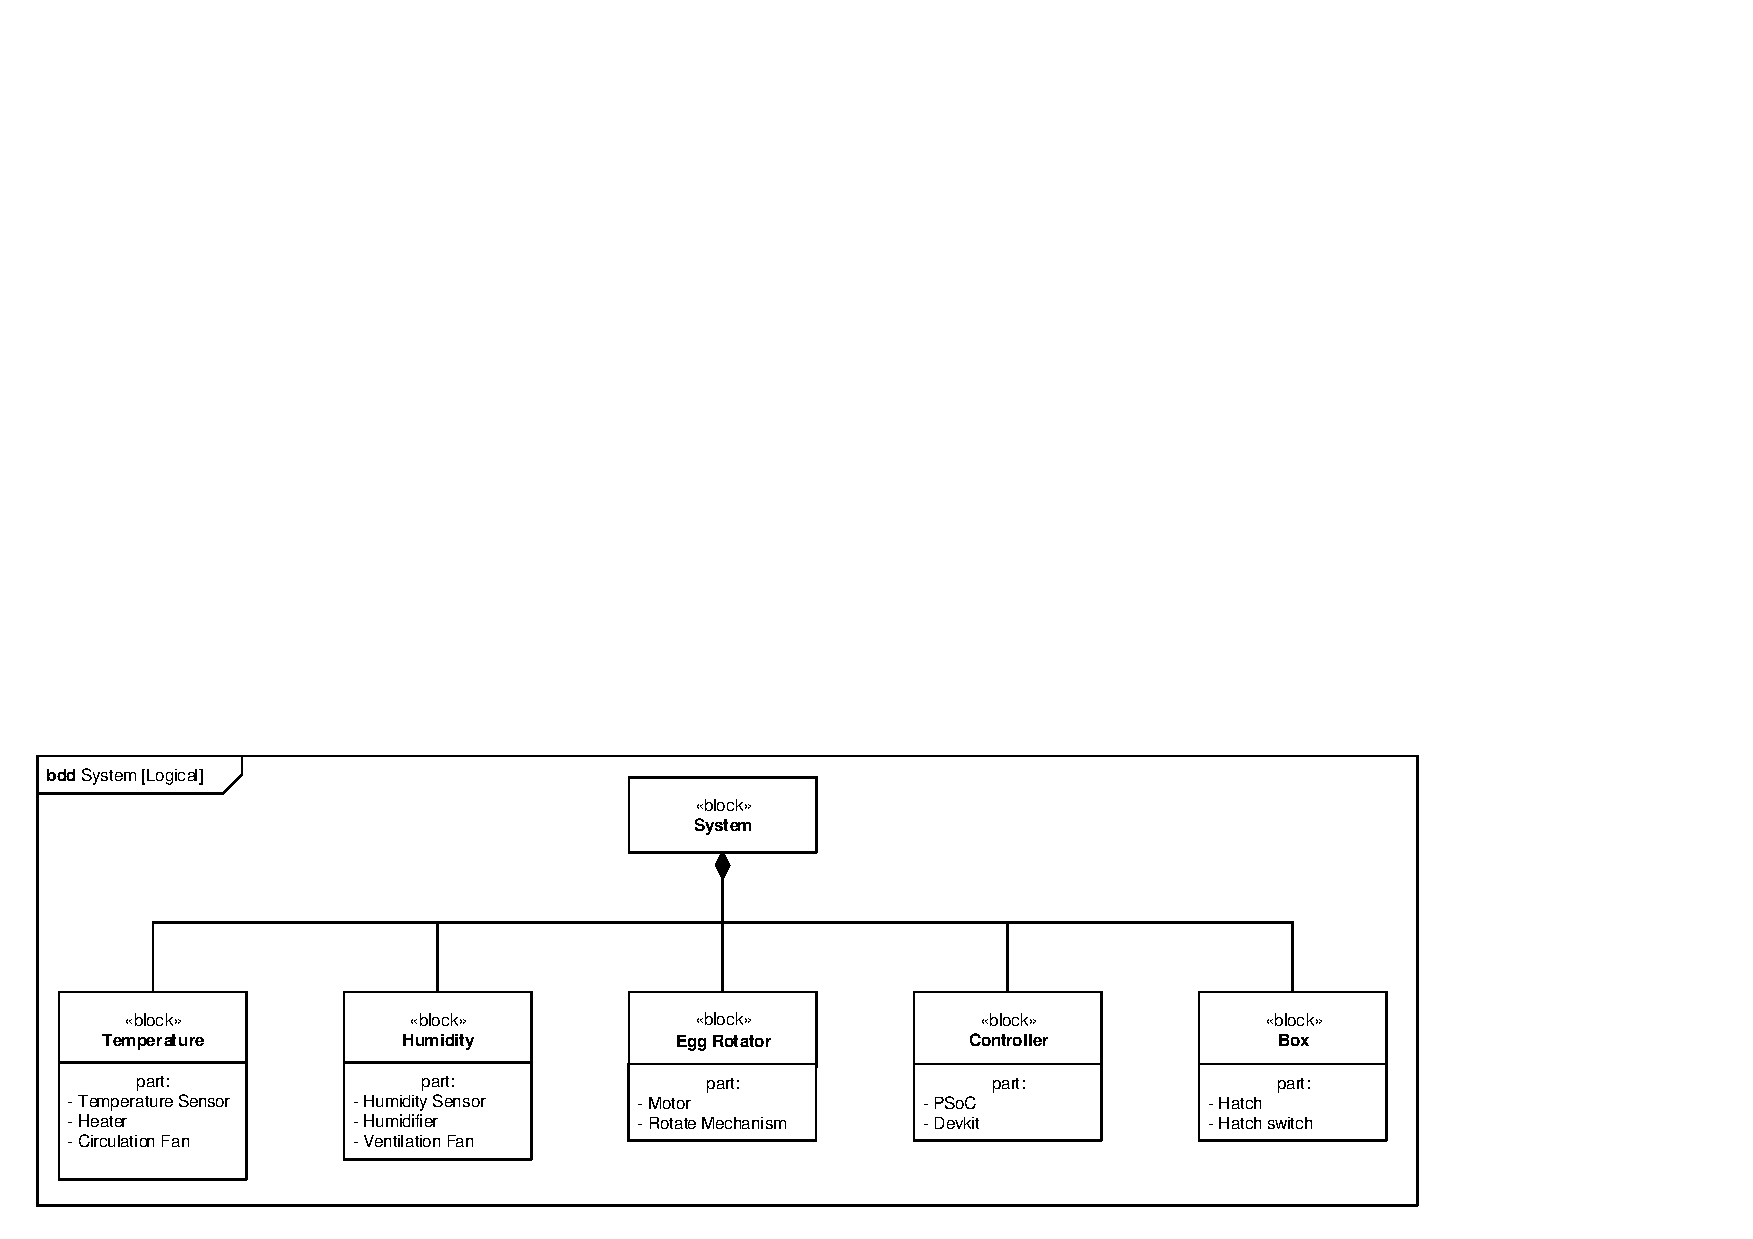
\includegraphics[page=1,width=\linewidth,viewport=08mm 8mm 238mm 80mm]{./5_systembeskrivelse/diagrammer/SYSML_Diagrammer_v4.pdf}
%\caption[Diagram]{Logical bdd}
%\label{fig:SystemStateDiagram}
%\end{figure}